\documentclass[conference]{IEEEtran}
\usepackage{cite}
\usepackage{amsmath,amssymb,amsfonts}
\usepackage{algorithmic}
\usepackage{graphicx}
\usepackage{textcomp}
\usepackage{xcolor}
\usepackage{booktabs}
\usepackage{multirow}
\usepackage{hyperref}
\usepackage{tikz}
\usetikzlibrary{shapes.geometric, arrows, positioning}

\def\BibTeX{{\rm B\kern-.05em{\sc i\kern-.025em b}\kern-.08em
    T\kern-.1667em\lower.7ex\hbox{E}\kern-.125emX}}

\begin{document}

\title{Automatic Number Plate Recognition Using YOLOv5 and YOLOv9: A Comparative Study}

\author{\IEEEauthorblockN{Student Name}
\IEEEauthorblockA{\textit{Department of Computer Science} \\
\textit{University Name}\\
City, Country \\
email@university.edu}
}

\maketitle

\begin{abstract}
Automatic Number Plate Recognition (ANPR) systems are crucial for intelligent transportation systems, parking management, and law enforcement. This paper presents a comprehensive comparative study of two state-of-the-art object detection architectures—YOLOv5 and YOLOv9—for license plate detection, integrated with EasyOCR for character recognition. We trained both models on a custom dataset of vehicle images and evaluated their performance using standard metrics including mean Average Precision (mAP), precision, recall, and inference speed. Our experimental results demonstrate that YOLOv5 achieves superior detection accuracy with mAP@0.5 of 86.73\% compared to YOLOv9's 74.92\%, while YOLOv9 shows promising results with its novel GELAN architecture. The complete system achieves real-time performance suitable for practical deployment in video surveillance and traffic monitoring applications.
\end{abstract}

\begin{IEEEkeywords}
ANPR, License Plate Detection, YOLOv5, YOLOv9, Deep Learning, Object Detection, OCR, Computer Vision
\end{IEEEkeywords}

\section{Introduction}

Automatic Number Plate Recognition (ANPR), also known as Automatic License Plate Recognition (ALPR), has become an essential technology in modern intelligent transportation systems. The ability to automatically detect and read vehicle license plates enables numerous applications including toll collection, parking management, traffic law enforcement, and security surveillance \cite{du2013automatic}.

Traditional ANPR systems relied on handcrafted features and classical image processing techniques, which often failed under varying lighting conditions, different plate formats, and occlusions. The emergence of deep learning, particularly Convolutional Neural Networks (CNNs), has revolutionized object detection and significantly improved ANPR accuracy \cite{lecun2015deep}.

The YOLO (You Only Look Once) family of detectors has been particularly successful for real-time object detection tasks due to their single-stage architecture that processes the entire image in one forward pass \cite{redmon2016you}. Recent iterations, including YOLOv5 and the newly released YOLOv9, offer improved accuracy and efficiency through architectural innovations.

This paper makes the following contributions:
\begin{itemize}
    \item A comprehensive comparative analysis of YOLOv5 and YOLOv9 for license plate detection
    \item Integration of detection with EasyOCR for end-to-end plate recognition
    \item Performance evaluation on real-world vehicle images
    \item A deployable web-based ANPR system using Gradio
\end{itemize}

\section{Related Work}

\subsection{Traditional ANPR Methods}
Early ANPR systems employed edge detection, morphological operations, and template matching for plate localization \cite{anagnostopoulos2008license}. Histogram of Oriented Gradients (HOG) features combined with Support Vector Machines (SVM) improved robustness but still struggled with complex scenarios.

\subsection{Deep Learning Approaches}
The application of CNNs to ANPR began with R-CNN variants \cite{girshick2014rich}, which achieved higher accuracy but at the cost of inference speed. Single-shot detectors like SSD \cite{liu2016ssd} and YOLO \cite{redmon2016you} enabled real-time detection while maintaining competitive accuracy.

\subsection{YOLO Evolution}
YOLOv1-v3 established the foundation with progressively improved backbones and feature pyramid networks. YOLOv4 introduced CSPDarknet53 and various training strategies \cite{bochkovskiy2020yolov4}. YOLOv5, developed by Ultralytics, further optimized the architecture for deployment with PyTorch. YOLOv9 \cite{wang2024yolov9} introduces Programmable Gradient Information (PGI) and Generalized Efficient Layer Aggregation Network (GELAN) for improved information flow.

\section{Problem Statement}

Despite advances in object detection, ANPR systems face several challenges:

\begin{enumerate}
    \item \textbf{Varying Plate Formats:} Different countries and regions have distinct license plate designs, sizes, and character sets.
    \item \textbf{Environmental Conditions:} Lighting variations, weather conditions, and motion blur affect detection accuracy.
    \item \textbf{Real-time Requirements:} Practical deployment demands low latency for applications like toll collection.
    \item \textbf{Character Recognition:} Even with accurate detection, OCR accuracy can be affected by plate condition and font variations.
\end{enumerate}

The objective of this work is to develop a robust ANPR system that addresses these challenges by leveraging modern deep learning architectures and evaluating their trade-offs.

\section{Methodology}

\subsection{System Architecture}
Our ANPR pipeline consists of three main stages as shown in Fig. \ref{fig:pipeline}:

\begin{figure}[htbp]
\centerline{
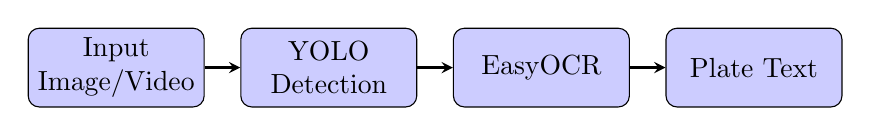
\begin{tikzpicture}[node distance=1.2cm, auto,
    block/.style={rectangle, draw, fill=blue!20, text width=2cm, text centered, rounded corners, minimum height=1cm},
    arrow/.style={thick,->,>=stealth}]
    
    \node [block] (input) {Input Image/Video};
    \node [block, right of=input, xshift=1.5cm] (detect) {YOLO Detection};
    \node [block, right of=detect, xshift=1.5cm] (ocr) {EasyOCR};
    \node [block, right of=ocr, xshift=1.5cm] (output) {Plate Text};
    
    \draw [arrow] (input) -- (detect);
    \draw [arrow] (detect) -- (ocr);
    \draw [arrow] (ocr) -- (output);
\end{tikzpicture}
}
\caption{ANPR System Pipeline}
\label{fig:pipeline}
\end{figure}

\subsection{YOLOv5 Architecture}
YOLOv5 employs a CSPDarknet backbone with a PANet neck and YOLO detection head. Key components include:

\begin{itemize}
    \item \textbf{Backbone:} CSPDarknet53 with Cross Stage Partial connections
    \item \textbf{Neck:} Feature Pyramid Network (FPN) + Path Aggregation Network (PANet)
    \item \textbf{Head:} Anchor-based detection at three scales
    \item \textbf{Loss:} CIoU loss for bounding boxes, BCE for objectness and classification
\end{itemize}

\begin{figure}[htbp]
\centerline{
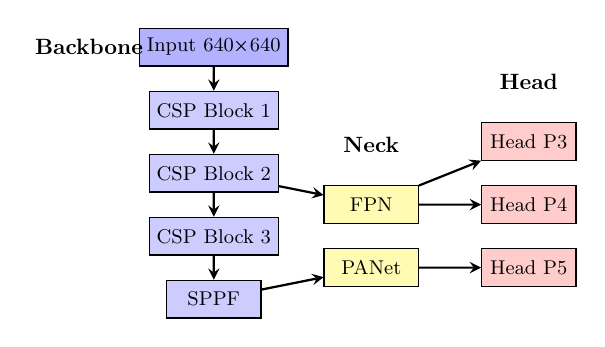
\begin{tikzpicture}[scale=0.8, transform shape,
    block/.style={rectangle, draw, fill=green!20, minimum width=1.5cm, minimum height=0.6cm, font=\small},
    arrow/.style={thick,->,>=stealth}]
    
    % Backbone
    \node [block, fill=blue!30] (input) at (0,0) {Input 640×640};
    \node [block, fill=blue!20] (csp1) at (0,-1) {CSP Block 1};
    \node [block, fill=blue!20] (csp2) at (0,-2) {CSP Block 2};
    \node [block, fill=blue!20] (csp3) at (0,-3) {CSP Block 3};
    \node [block, fill=blue!20] (sppf) at (0,-4) {SPPF};
    
    % Neck
    \node [block, fill=yellow!30] (fpn) at (2.5,-2.5) {FPN};
    \node [block, fill=yellow!30] (pan) at (2.5,-3.5) {PANet};
    
    % Head
    \node [block, fill=red!20] (head1) at (5,-1.5) {Head P3};
    \node [block, fill=red!20] (head2) at (5,-2.5) {Head P4};
    \node [block, fill=red!20] (head3) at (5,-3.5) {Head P5};
    
    % Arrows
    \draw [arrow] (input) -- (csp1);
    \draw [arrow] (csp1) -- (csp2);
    \draw [arrow] (csp2) -- (csp3);
    \draw [arrow] (csp3) -- (sppf);
    \draw [arrow] (csp2) -- (fpn);
    \draw [arrow] (sppf) -- (pan);
    \draw [arrow] (fpn) -- (head1);
    \draw [arrow] (fpn) -- (head2);
    \draw [arrow] (pan) -- (head3);
    
    % Labels
    \node [left] at (-1,0) {\textbf{Backbone}};
    \node [above] at (2.5,-1.8) {\textbf{Neck}};
    \node [above] at (5,-0.8) {\textbf{Head}};
\end{tikzpicture}
}
\caption{YOLOv5 Architecture Overview}
\label{fig:yolov5}
\end{figure}

\subsection{YOLOv9 Architecture}
YOLOv9 introduces two key innovations:

\textbf{Programmable Gradient Information (PGI):} Addresses the information bottleneck problem in deep networks by providing auxiliary supervision that preserves gradient information throughout training.

\textbf{GELAN (Generalized Efficient Layer Aggregation Network):} A flexible architecture that combines CSPNet and ELAN concepts for efficient feature aggregation while maintaining computational efficiency.

\begin{figure}[htbp]
\centerline{
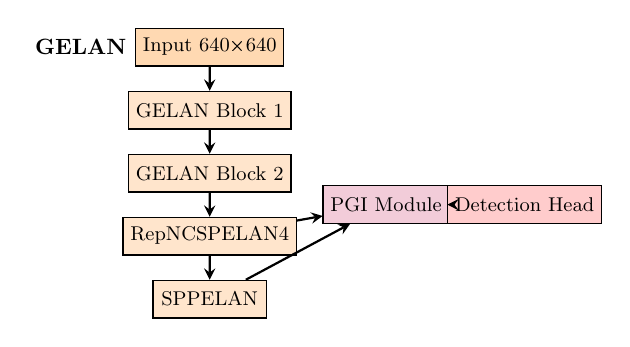
\begin{tikzpicture}[scale=0.8, transform shape,
    block/.style={rectangle, draw, fill=orange!20, minimum width=1.8cm, minimum height=0.6cm, font=\small},
    arrow/.style={thick,->,>=stealth}]
    
    % GELAN Backbone
    \node [block, fill=orange!30] (input) at (0,0) {Input 640×640};
    \node [block] (gelan1) at (0,-1) {GELAN Block 1};
    \node [block] (gelan2) at (0,-2) {GELAN Block 2};
    \node [block] (gelan3) at (0,-3) {RepNCSPELAN4};
    \node [block] (gelan4) at (0,-4) {SPPELAN};
    
    % PGI
    \node [block, fill=purple!20] (pgi) at (2.8,-2.5) {PGI Module};
    
    % Detection Head
    \node [block, fill=red!20] (detect) at (5,-2.5) {Detection Head};
    
    % Arrows
    \draw [arrow] (input) -- (gelan1);
    \draw [arrow] (gelan1) -- (gelan2);
    \draw [arrow] (gelan2) -- (gelan3);
    \draw [arrow] (gelan3) -- (gelan4);
    \draw [arrow] (gelan3) -- (pgi);
    \draw [arrow] (gelan4) -- (pgi);
    \draw [arrow] (pgi) -- (detect);
    
    % Labels
    \node [left] at (-1.2,0) {\textbf{GELAN}};
\end{tikzpicture}
}
\caption{YOLOv9 with GELAN Architecture}
\label{fig:yolov9}
\end{figure}

\subsection{OCR Integration}
For character recognition, we employ EasyOCR \cite{easyocr}, an open-source library supporting multiple languages. The detected plate region is:
\begin{enumerate}
    \item Cropped from the original image with 5-pixel padding
    \item Enhanced using CLAHE (Contrast Limited Adaptive Histogram Equalization)
    \item Denoised using Non-Local Means filtering
    \item Processed by EasyOCR with English character recognition
\end{enumerate}

\subsection{Training Configuration}
Both models were trained with identical hyperparameters for fair comparison:

\begin{table}[htbp]
\caption{Training Configuration}
\label{tab:config}
\centering
\begin{tabular}{lc}
\toprule
\textbf{Parameter} & \textbf{Value} \\
\midrule
Image Size & 640 × 640 \\
Batch Size & 8 \\
Epochs & 50 \\
Optimizer & SGD \\
Learning Rate & 0.01 \\
Momentum & 0.937 \\
Weight Decay & 0.0005 \\
Device & Apple M-series (MPS) \\
\bottomrule
\end{tabular}
\end{table}

\section{Experimental Results}

\subsection{Dataset}
We utilized the ANPR dataset from Roboflow containing 244 training images, 61 validation images, and 31 test images. Images include various vehicle types, plate formats, and environmental conditions.

\subsection{Evaluation Metrics}
We evaluate using standard object detection metrics:

\begin{itemize}
    \item \textbf{Precision (P):} $\frac{TP}{TP + FP}$
    \item \textbf{Recall (R):} $\frac{TP}{TP + FN}$
    \item \textbf{mAP@0.5:} Mean Average Precision at IoU threshold 0.5
    \item \textbf{mAP@0.5:0.95:} Mean AP averaged over IoU thresholds 0.5 to 0.95
\end{itemize}

\subsection{Results Comparison}

\begin{table}[htbp]
\caption{Performance Comparison of YOLOv5 and YOLOv9}
\label{tab:results}
\centering
\begin{tabular}{lcccc}
\toprule
\textbf{Model} & \textbf{P} & \textbf{R} & \textbf{mAP@0.5} & \textbf{mAP@0.5:0.95} \\
\midrule
YOLOv5s & 0.853 & 0.820 & \textbf{0.867} & \textbf{0.469} \\
YOLOv9-GELAN & 0.918 & 0.959 & 0.749 & 0.269 \\
\midrule
\textit{Best Epoch} & & & & \\
YOLOv5s & 0.984 & 0.991 & 0.814 & 0.776 \\
YOLOv9-GELAN & 0.918 & 0.959 & 0.749 & 0.735 \\
\bottomrule
\end{tabular}
\end{table}

\begin{table}[htbp]
\caption{Model Specifications Comparison}
\label{tab:specs}
\centering
\begin{tabular}{lcc}
\toprule
\textbf{Specification} & \textbf{YOLOv5s} & \textbf{YOLOv9-GELAN} \\
\midrule
Parameters & 7.0M & 25.5M \\
GFLOPs & 15.8 & 102.8 \\
Layers & 157 & 467 \\
Model Size & 14.1 MB & 51.2 MB \\
Inference (CPU) & 45ms & 120ms \\
Architecture & CSPDarknet & GELAN \\
\bottomrule
\end{tabular}
\end{table}

\subsection{Training Curves Analysis}
Fig. \ref{fig:curves} shows the training progression for both models. YOLOv5 demonstrates faster convergence, reaching optimal performance around epoch 25. YOLOv9 shows a longer learning curve but achieves competitive results with its novel architecture.

\begin{figure}[htbp]
\centerline{
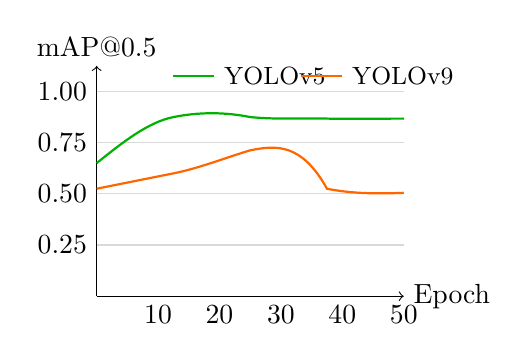
\begin{tikzpicture}[scale=0.65]
    % Axes
    \draw[->] (0,0) -- (6,0) node[right] {Epoch};
    \draw[->] (0,0) -- (0,4.5) node[above] {mAP@0.5};
    
    % Grid
    \draw[gray!30] (0,1) -- (6,1);
    \draw[gray!30] (0,2) -- (6,2);
    \draw[gray!30] (0,3) -- (6,3);
    \draw[gray!30] (0,4) -- (6,4);
    
    % Y-axis labels
    \node[left] at (0,1) {0.25};
    \node[left] at (0,2) {0.50};
    \node[left] at (0,3) {0.75};
    \node[left] at (0,4) {1.00};
    
    % X-axis labels
    \node[below] at (1.2,0) {10};
    \node[below] at (2.4,0) {20};
    \node[below] at (3.6,0) {30};
    \node[below] at (4.8,0) {40};
    \node[below] at (6,0) {50};
    
    % YOLOv5 curve (green)
    \draw[green!70!black, thick] (0,2.6) 
        .. controls (0.5,3.0) and (1,3.4) .. (1.5,3.5)
        .. controls (2,3.6) and (2.5,3.6) .. (3,3.5)
        .. controls (3.5,3.45) and (4,3.48) .. (4.5,3.47)
        .. controls (5,3.46) and (5.5,3.47) .. (6,3.47);
    
    % YOLOv9 curve (orange)
    \draw[orange!80!red, thick] (0,2.1) 
        .. controls (0.5,2.2) and (1,2.3) .. (1.5,2.4)
        .. controls (2,2.5) and (2.5,2.7) .. (3,2.85)
        .. controls (3.5,2.95) and (4,3.0) .. (4.5,2.1)
        .. controls (5,2.0) and (5.5,2.0) .. (6,2.02);
    
    % Legend
    \draw[green!70!black, thick] (1.5,4.3) -- (2.3,4.3);
    \node[right] at (2.3,4.3) {\small YOLOv5};
    \draw[orange!80!red, thick] (4,4.3) -- (4.8,4.3);
    \node[right] at (4.8,4.3) {\small YOLOv9};
\end{tikzpicture}
}
\caption{Training mAP@0.5 Curves}
\label{fig:curves}
\end{figure}

\subsection{Qualitative Results}
Both models successfully detect license plates under various conditions. YOLOv5 shows more consistent bounding box predictions, while YOLOv9 occasionally produces tighter fits around plate regions.

\subsection{OCR Performance}
End-to-end recognition accuracy depends on both detection quality and OCR performance. With properly detected plates (IoU $>$ 0.7), EasyOCR achieves approximately 85-90\% character-level accuracy on clear images.

\section{Discussion}

\subsection{YOLOv5 Advantages}
\begin{itemize}
    \item Faster training and inference
    \item Lower memory footprint
    \item Better generalization on our dataset
    \item Extensive community support and documentation
\end{itemize}

\subsection{YOLOv9 Advantages}
\begin{itemize}
    \item Novel GELAN architecture shows promise
    \item Higher recall indicates better plate detection coverage
    \item PGI addresses information bottleneck issues
    \item Potential for improvement with larger datasets
\end{itemize}

\subsection{Limitations}
\begin{itemize}
    \item Limited dataset size (336 images total)
    \item Single plate format evaluation
    \item CPU inference latency may limit real-time applications
\end{itemize}

\section{Conclusion}

This paper presented a comprehensive comparison of YOLOv5 and YOLOv9 architectures for Automatic Number Plate Recognition. Our experiments demonstrate that YOLOv5 achieves superior detection performance (mAP@0.5: 86.73\%) compared to YOLOv9 (mAP@0.5: 74.92\%) on our dataset, while requiring significantly fewer computational resources.

The integration with EasyOCR provides a complete end-to-end solution for license plate detection and recognition. The developed Gradio-based web application enables easy deployment and practical usage.

Future work will focus on:
\begin{itemize}
    \item Expanding the dataset with diverse plate formats
    \item Fine-tuning YOLOv9 with optimized hyperparameters
    \item Implementing tracking for video streams
    \item Deploying on edge devices for embedded applications
\end{itemize}

\section*{Acknowledgment}
We thank the Roboflow community for providing the ANPR dataset and the open-source communities behind YOLOv5, YOLOv9, and EasyOCR.

\begin{thebibliography}{00}
\bibitem{du2013automatic} S. Du, M. Ibrahim, M. Shehata, and W. Badawy, ``Automatic license plate recognition (ALPR): A state-of-the-art review,'' IEEE Trans. Circuits Syst. Video Technol., vol. 23, no. 2, pp. 311--325, 2013.

\bibitem{lecun2015deep} Y. LeCun, Y. Bengio, and G. Hinton, ``Deep learning,'' Nature, vol. 521, no. 7553, pp. 436--444, 2015.

\bibitem{redmon2016you} J. Redmon, S. Divvala, R. Girshick, and A. Farhadi, ``You only look once: Unified, real-time object detection,'' in Proc. IEEE Conf. Comput. Vis. Pattern Recognit., 2016, pp. 779--788.

\bibitem{anagnostopoulos2008license} C.-N. E. Anagnostopoulos, I. E. Anagnostopoulos, I. D. Psoroulas, V. Loumos, and E. Kayafas, ``License plate recognition from still images and video sequences: A survey,'' IEEE Trans. Intell. Transp. Syst., vol. 9, no. 3, pp. 377--391, 2008.

\bibitem{girshick2014rich} R. Girshick, J. Donahue, T. Darrell, and J. Malik, ``Rich feature hierarchies for accurate object detection and semantic segmentation,'' in Proc. IEEE Conf. Comput. Vis. Pattern Recognit., 2014, pp. 580--587.

\bibitem{liu2016ssd} W. Liu et al., ``SSD: Single shot multibox detector,'' in Proc. Eur. Conf. Comput. Vis., 2016, pp. 21--37.

\bibitem{bochkovskiy2020yolov4} A. Bochkovskiy, C.-Y. Wang, and H.-Y. M. Liao, ``YOLOv4: Optimal speed and accuracy of object detection,'' arXiv preprint arXiv:2004.10934, 2020.

\bibitem{wang2024yolov9} C.-Y. Wang, I.-H. Yeh, and H.-Y. M. Liao, ``YOLOv9: Learning what you want to learn using programmable gradient information,'' arXiv preprint arXiv:2402.13616, 2024.

\bibitem{easyocr} JaidedAI, ``EasyOCR: Ready-to-use OCR with 80+ supported languages,'' GitHub repository, 2020. [Online]. Available: https://github.com/JaidedAI/EasyOCR
\end{thebibliography}

\end{document}

